\chapter{THE LAWS OF VARIETY}\label{THE LAWS OF VARIETY}
%\addcontentsline{toc}{chapter}{Appendix 2. THE LAWS OF VARIETY}
\section*{Overview}
\begin{center}
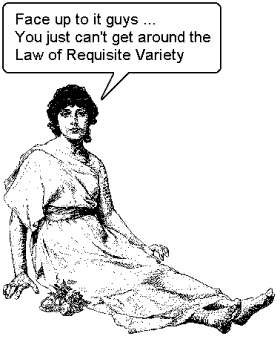
\includegraphics[max width=\textwidth]{sitting3}
\end{center}

The various parts of any system have to be in balance.

Some design procedure is essential in order to ensure that an engine is in balance with the vehicle it drives, or that the heart is designed with sufficient capacity to pump the blood around the organism.

In organisational terms, this (for example) concerns ensuring that the capabilities of the systems which regulate are sufficient to deal with the complexity of the problems which they have to deal with.

Variety is the cybernetician's tool with dealing with these issues.

It's the only method I've so far encountered which encourages you to consider a wide range of solutions and to avoid the knee-jerk reaction of "Well it's obvious ... we need more managers."

\section*{THE LAWS OF VARIETY - WHY BOTHER?}
There is nothing which puts people off VSM ideas quicker than the Laws of Variety. I've met dozens of people who picked up Stafford's books and after a couple of hours put them down in bewilderment and never got any further.

So for those of you who have found yourselves in this position, please consider

\begin{itemize}
  \item Yes, these ideas are new and strange and a little hard to grasp.

  \item There are ways of thinking about all of this which make it easier.

  \item It's worth the effort.

\end{itemize}

All of the crucial aspects of VSM diagnosis and design come from working with variety. The overall vision of self managed, autonomous work-groups and the job of the Metasystem as \textbf{cohesion} comes straight from the variety engineering.

The issue is one of balance. The bits of the VSM have now been discussed and (if you are doing the exercises) identified for your particular enterprise. But what now? You have your Operational elements, and some aspects of systems 2, 3, 4 and 5, but how do you know if the system as a whole is properly designed?

For example, if you've identified System Four as a planning meeting which is held once a year, its highly unlikely that this can carry out the job of ensuring your enterprise can respond to a changing environment. What happens if an opportunity arises? Will you have to wait several months to do something about it? In this case it looks highly likely that your design for a System Four is inadequate, that is, it's \textit{out of balance} with the rest of the structure.

In balancing the parts of you enterprise and (just as importantly) ensuring that your enterprise is in ecological balance with its environment, the following questions must be answered:

\begin{itemize}
  \item Do the operational elements have the ability to respond to changes in their environment?

  \item Do Systems 2 and 3 have the capabilities to carry out their functions of dealing with the inside and now of the enterprise?

  \item Is System 4 designed to be in balance with its internal environment and to deal with the accelerating rate of change in the external environment?

  \item Do the Policy systems work? Are they adequately informed? Are they poised to intervene when necessary?

\end{itemize}

These questions are answered most appropriately by thinking in terms of variety.

\section*{INTRODUCING VARIETY}
The definition of variety is straightforward. It is the number of states in which a system can exist. A switch has a variety of two (on and off) a child has a variety which is enormous.


\section*{VARIETY BALANCES - ASHBY'S LAW}
Consider a steam engine under the control of a Watt governor.

The engine speeds up, the balls fly out, the steam supplied to the engine is cut down. The engine slows down, the balls retract, more steam is let in, the engine speeds up, the balls fly out, and round we go.

It's just the same as a thermostat, or any regulatory device. The Governor is charged with the regulation (control, management) of another system. What can we conclude from all of this?

The complexity of steam engine is defined as the number of possible states in which it can exist. This will mainly be concerned with the different speeds at which it can run, and it will be huge.

In designing the regulator it obvious that it must be able to respond to every state of the engine. (State 23,721, let in 34\% more steam. ... State 349,856 cut down the steam by 56\% ... ) and so on.

In every case, its essential that the regulator can respond to every state in which the steam engine can exist. It would not work if it reached a particular speed which the regulator could not respond to. The system would fail.

So the variety of the Watt Governor must be at least as large as the variety of the steam engine. And in more general terms:

\textbf{\textit{"The variety of a regulator must be at least as large as that of the system it regulates"}}

This statement is usually referred to as \textbf{\href{https://vsmg.lrc.org.uk/screen.php?page=bibliography}{Ashby's Law of Requisite Variety}}, as it says that the regulator must have enough (requisite) variety to adequately do its job.

Assuming that this is clear in the case of the Watt Governor, consider a game of table tennis. Both players have similar variety (they are of similar standards) and each controls the other. The varieties are matched. If one takes lessons, and learns several new techniques, he will increase his variety and the other player will not have enough (requisite) variety to control him.

The other player - who happens to be a cybernetician - thinks "I really have to amplify my variety ... you just can't get around Ashby's's law of Requisite variety!"

And note that while its unlikely that any one table tennis champion would have the variety to beat three simultaneous opponents, chess grand-masters can amplify their variety to such an extent they can match the variety of dozens of opponents.

\section*{OBVIOUS WAYS OF BALANCING VARIETY}
So far we have seen that

\begin{itemize}
  \item variety is a measure of complexity

  \item for a system to work, varieties must be in balance.

\end{itemize}

Some of this was hinted at in the \href{https://vsmg.lrc.org.uk/screen.php?page=2_2cs2}{Suma} case study.

The diagram represents a system where the Metasystem has enough variety to provide cohesion. Or, for every state the operation can exhibit, the Metasystem has the ability to respond. The Metasystem has enough or "requisite variety".

The other diagram showed a huge Operation (more stock lines, more customers, more people, and most importantly cataclysmic increases in permutations) due to exploding variety, and a simultaneous decrease in the size of the Metasystem. Requisite variety had been lost. So the Metasystemic didn't have the capacity to respond to every state of the Operation - it don't work properly. Conflicts were not resolved. No synergy. No forward planning. Policy no longer rounded off the system, so that people could ignore policy constraints.

So what can be done?

Varieties had to be rebalanced, and this can be done in two ways: the variety of the Metasystem can be increased, or the variety of the Operation can be limited.

The usual methods of exercising control are well known. Managers are given more powers and training, (more variety), or the options of Operational workers are restricted (less variety).


\section*{LESS OBVIOUS WAYS OF BALANCING VARIETY}
The power of Variety engineering begins to emerge at this point.p>

If the key is to balance the relative varieties of the Operation and the Metasystem, then new options can be considered.

\subsection*{\textit{Limiting Operational Variety by empowering the workforce}}
If the problem is the exploding variety of the Operation then one solution is to get the people working within the Operation to limit their own variety. Rather than impose an authoritarian regime, you could shrink the size of the Operational problem by getting the people actually doing the work to deal with the problems themselves. Thus self-management, worker empowerment and all the Tom Peters stuff about training production line staff to do statistical analysis of production figures.

"GRASP THIS NETTLE

The management of the system-in-focus is in principle unable to entertain the variety generated by any one (never mind all) of its subsidiary viable systems that constitute System One.

The beginnings of a theory of autonomy, of decentralisation lie in this simple fact"

(Beer "\href{https://vsmg.lrc.org.uk/screen.php?=bibliography}{Diagnosing the System}" p.37)

\subsection*{\textit{Balancing Varieties using Information Processing}}
The conclusion is encouraging: a well designed information system can be used as an alternative to authoritarian control. It can enhance self-managed, autonomous individuals.

\section*{A NEW UNIVERSE OF POSSIBILITIES}

\section*{DESIGN BY VARIETY ENGINEERING}
Variety engineering is the term used to describe the technique of looking at the multitude of ways that varieties can be manipulated in designing effective organisations.

The essence of this approach is to provide a set of tools (involving variety) which gives you a whole range of new options.

The trick is to find a way of skinning the cat, which does minimal harm to the cat.

"Managerial, operational and environmental varieties should be designed to balance, with minimal damage to people and to cost."

(Beer "\href{https://vsmg.lrc.org.uk/screen.php?=bibliography}{The Heart of Enterprise}" p.97)

This is a slightly abridged version of Beer's First Principle of Organisation. If it's accepted that you can choose between a philosophy involving bullies, soldiers, and blind obedience, or of working a new universe of possibilities including autonomy and carefully constructed information systems, then the way forward (for most of us) is clear.

Many of the basic premises of co-operation can be re-interpreted in this light. Basing an organisation on self-managed individuals, rather than the cog-in-machine vision of production line techniques, becomes a sound working practice in terms of variety engineering. The vast majority of problems are dealt with at this level, huge quantities of variety are absorbed by intelligent behaviour at the operational level, and the remaining problems ( sometimes called residual variety) can be mopped up easily by the Metasystem.

In more traditional terms the argument can be expressed as follows:

\textbf{\textit{"If you empower the workers to solve their own problems, then the people whose job it is to manage these workers will have almost nothing to do."}}

The politics of all this are endless. In terms of variety engineering its simply a question of deciding which of the many methods of balancing varieties are the most effective. Interestingly enough the most appropriate solutions generally seem to suggest more libertarian protocols.

\section*{SUMMARY}
Variety is a measure of complexity.

Ashby's Law states that the variety of a system which regulates has to equal the variety of the system it is regulating.

This can be expressed in a number of ways. It's often expressed as:

"Only Variety can absorb variety"

In organisational terms it means that the capabilities of the regulators, have to balance the complexity of the situation they are charged with regulating.

This regulation could be the traditional view of management, or it could be the regulation of a jazz band where the rules by which the music unfolds are under the control of the people making it. Or the regulation of body temperature. In all these cases Ashby's Law is pertinent.

If the systems which regulate don't have enough (or requisite) variety to match the complexity of the regulated, then regulation will fail. The system will be out of control.

Variety Engineering is the manipulation of varieties in whatever way is most appropriate to restore the balance between regulator and regulated.

In practical terms the consideration of organisational problems in terms of variety provides a huge new battery of possibilities which are unavailable to other techniques.

\textit{\textbf{Some level of understanding of these ideas is essential for the rest of this book. However, given the difficulty many people have with variety, I will usually include a re-interpretation using more conventional language.}}

If the entire concept leaves you completely bewildered, try re-reading this chapter or one of Beer's many introductions to variety (or the original treatment in \textbf{\href{https://vsmg.lrc.org.uk/screen.php?page=bibliography}{An Introduction to Cybernetics}} by \textbf{W. Ross Ashby} - Chapman and Hall, 1956). (The language used to write about systems has changed over the years but, despite that, this classic textbook is still as useful as ever. It was written to be accessible to as wide a variety of readers as possible and is still the only book to cover the fundamentals of cybernetics with a clear, step-by-step approach. In recognition of this book's importance, the \href{http://pespmc1.vub.ac.be/}{Principia Cybernetica Web} has made a \href{http://pespmc1.vub.ac.be/ASHBBOOK.html}{PDF version} available on-line.)
